% !TeX root=main.tex
\pagenumbering{arabic}
\chapter{مقدمه}
\thispagestyle{empty}
	در سال‌های اخیر پیشرفت‌های زیادی در مسائل هوش مصنوعی و یادگیری عمیق که در تقاطع دو حوزه پردازش زبان طبیعی  و بینایی ماشین  قرار می‌گیرند؛ رخ داده است. یکی از مسائلی که اخیراً مورد توجه قرارگرفته است؛ پرسش و پاسخ تصویری  است. با توجه به یک تصویر و یک سؤال به زبان طبیعی، سیستم سعی می‌کند با استفاده از عناصر بصری تصویر و استنتاج جمع آوری شده از سوال متنی، پاسخ صحیح را پیدا کند 
	\cite{manmadhan2020visual}.
	پرسش و پاسخ تصویری نسخه گسترش یافته مسئله پرسش و پاسخ متنی  است است که اطلاعات بصری به مسئله اضافه شده است. شکل \ref{fig:VQAExample}  گویای تفاوت این دو مسئله است.
	\begin{figure}
		\centerline{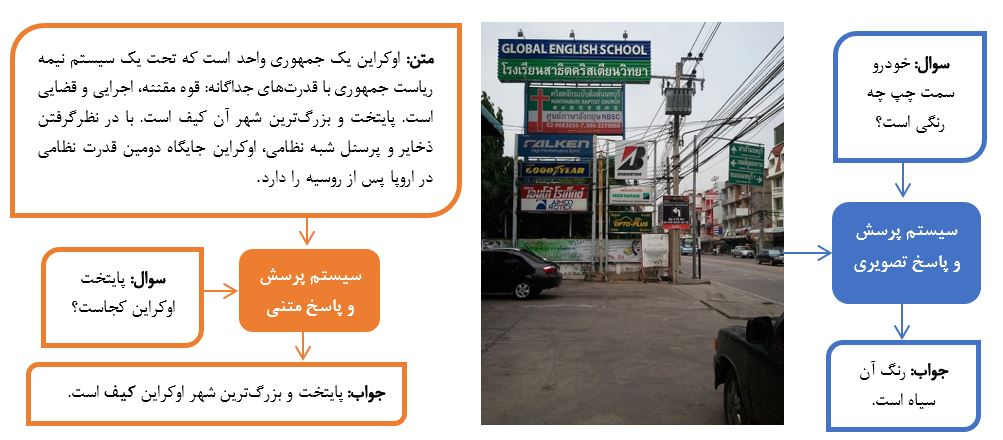
\includegraphics[scale=0.7]{images/1.JPG}}
		\caption{مثالی از سیستم پرسش و پاسخ متنی و تصویری}
		\label{fig:VQAExample}
	\end{figure}
	
	در سیستم پرسش و پاسخ متنی، یک متن و یک سوال متنی به عنوان ورودی به سیستم داده می‌شود و انتظار می‌رود که سیستم با توجه به درک و تفسیری که از متن و سوال بدست می‌آورد؛ یک جواب متنی را خروجی دهد. اما در سیستم پرسش و پاسخ تصویری، یک تصویر و یک سوال متنی به ورودی سیستم داده می‌شود و انتظار می‌رود که سیستم بتواند با استفاده از عناصر بصری تصویر و تفسیری که از سوال بدست می‌آورد؛ یک پاسخ متنی را در خروجی نشان دهد.
	
	مسئله پرسش و پاسخ تصویری پیچیدگی بیشتری نسبت به مسئله پرسش و پاسخ متنی دارد زیرا تصاویر بعد بالاتر و نویز بیشتری نسبت به متن دارند. علاوه بر این، تصاویر فاقد ساختار و قواعد دستوری زبان هستند. در نهایت هم، تصاویر غنای بیشتری از دنیای واقعی را ضبط می‌کنند، در حالی که زبان طبیعی در حال حاضر نشانگر سطح بالاتری از انتزاع دنیای واقعی است
	\cite{wu2017visual}.
	

\section{کاربرد و اهمیت مسئله}
	در طی سال‌های متمادی، محققان به دنبال ساخت ماشین‌هایی بودند که به اندازه‌ی کافی باهوش باشند که از آن به طور موثر همانند انسان‌ها برای تعامل استفاده کنند. مسئله‌ی پرسش و پاسخ تصویری یکی از پله‌های رسیدن به این رویای هوش مصنوعی است و از این جهت حائز اهمیت است.

	کاربردهای بسیاری برای پرسش و پاسخ تصویری وجود دارد. یکی از مهم‌ترین موارد دستیار هوشمند برای افراد کم‌بینا و نابینا  است
	\cite{gurari2018vizwiz}.
	علاوه بر این، در سال های اخیر دستیاران صوتی
 	\footnote{\lr{Voice Assistants}}
   و عامل‌های گفتگو
    \footnote{\lr{Conversational Agents}}
     مانند  
	\lr{Cortana}
	،
	\lr{Siri}
و
	\lr{Alexa}
	در بازار عرضه شدند که می‌توانند با انسان‌ها با استفاده از زبان طبیعی ارتباط برقرار کنند. در حال حاضر این دستیاران با استفاده از صوت و متن این ارتباط را برقرار می‌کنند در نتیجه گفتگوی بین این دستیاران با انسان‌ها مشابه دنیای واقعی نمی‌باشد. این ارتباط را می‌توان با استفاده از داده‌های تصویری و ویدئویی به واقعیت نزدیک‌تر کرد. اینجاست که مسئله‌ی پرسش و پاسخ تصویری برای نزدیک کردن تعامل بین انسان و عامل‌های گفتگو به دنیای واقعی می‌تواند موثر باشد.  همین موضوع را می‌توانیم به صورت گسترده‌تری در ربات‌ها مشاهده کنیم. برای این‌که ربات بتواند بهتر با انسان‌ها ارتباط برقرار کند و به سوالات و درخواست‌ها پاسخ دهد؛ نیاز دارد که درک و فهم درستی از اطراف داشته باشد که این مستلزم داشتن تصویری دقیق از پیرامون است. بنابراین این ربات می‌تواند برای پاسخ به پرسش‌ها از دانشی که از طریق تصویر پیرامون خود بدست می‌آورد، جواب درستی را بدهد. 
  
  کاربرد دیگر این مسئله در پزشکی است. در بسیاری از موارد تحلیل تصاویر پزشکی مانند تصاویر
   \lr{CT}
   ‌ اسکن و 
   \lr{x-ray}
   برای یک پزشک متخصص هم دشوار است. اما یک سیستم پرسش و پاسخ تصویری می‌تواند با تحلیل و تشخیص موارد غیرطبیعی موجود در تصویر، به عنوان نظر دوم به پزشک متخصص کمک کند. از طرفی ممکن است در بعضی اوقات بیمار دسترسی به پزشک را نداشته باشد تا شرح تصاویر را متوجه شود. وجود سیستم پرسش و پاسخ تصویری می‌تواند آگاهی بیمار را نسبت به بیماری افزایش دهد و از نگرانی او بکاهد
   \cite{talafha2018just}.

\section{بررسی چالش‌های موجود در این مسئله}
	در مقایسه با مسائل دیگری که مشترک بین پردازش زبان طبیعی و بینایی ماشین است مانند توصیف تصویر
	\footnote{\lr{Image Captioning}}
	و بازیابی متن به تصویر
	\footnote{\lr{Text-to-image Retrieval}}
	، مسئله پرسش و پاسخ تصویری چالش‌برانگیزتر است زیرا (1)  سوالات از پیش تعیین نشده است. به این معنی که در مسئله‌ای مانند تشخیص اشیا، سوال این است که چه اشیایی در تصویر وجود دارد و این سوال از پیش تعیین شده است و در طول حل مسئله تغییر نمی‌کند و تنها تصویر تغییر می‌کند که منجر به پاسخ‌ها متفاوت می‌شود. اما در پرسش و پاسخ تصویری، برای هر تصویر سوالات متفاوت و مرتبط با همان تصویر پرسیده می‌شود که در زمان اجرا تعیین می‌شود. (2) اطلاعات موجود در تصویر ابعاد بالایی دارد که پردازش آن‌ها به زمان و حافظه زیادی نیاز دارد. (3) مسئله پرسش و پاسخ تصویری نیاز به حل مسائل پایه‌ای  و فرعی دارد مانند تشخیص اشیا
	\footnote{\lr{Object Detection}}
	(آیا در تصویر سگ وجود دارد؟)، تشخیص فعالیت
	\footnote{\lr{Activity Recognition}}
	(آیا کودک گریه می‌کند؟)، طبقه‌بندی صفات
	\footnote{\lr{Attribute Classification}}
	(چتر چه رنگی است؟)، شمارش(چند نفر در تصویر وجود دارد؟)، طبقه‌بندی صحنه
	\footnote{\lr{Scene Classification}}
	(هوا بارانی است؟) و روابط مکانی بین اشیا(چه چیزی بین گربه و مبل است؟).

